% The document class supplies options to control rendering of some standard
% features in the result.  The goal is for uniform style, so some attention 
% to detail is *vital* with all fields.  Each field (i.e., text inside the
% curly braces below, so the MEng text inside {MEng} for instance) should 
% take into account the following:
%
% - author name       should be formatted as "FirstName LastName"
%   (not "Initial LastName" for example),
% - supervisor name   should be formatted as "Title FirstName LastName"
%   (where Title is "Dr." or "Prosddeseseesdeswsedwqf." for example),
% - degree programme  should be "BSc", "MEng", "MSci", "MSc" or "PhD",
% - dissertation title should be correctly capitalised (plus you can have
%   an optional sub-title if appropriate, or leave this field blank),
% - dissertation type should be formatted as one of the following:
%   * for the MEng degree programme either "enterprise" or "research" to
%     reflect the stream,
%   * for the MSc  degree programme "$X/Y/Z$" for a project deemed to be
%     X%, Y% and Z% of type I, II and III.
% - year              should be formatted as a 4-digit year of submission
%   (so 2014 rather than the accademic year, say 2013/14 say).

\documentclass[ % the name of the author
                    author={Jonathan Rankin},
                % the name of the supervisor
                supervisor={Dr. David May, Dr. Ian Holyer},
                % the degree programme
                    degree={MEng},
                % the dissertation    title (which cannot be blank)
                     title={CodeTouch},
                % the dissertation subtitle (which can    be blank)
                  subtitle={A Revolutionary Way To Program Real Code On Touch Screen Devices},
                % the dissertation     type
                      type={enterprise},
                % the year of submission
                      year={2015 } ]{dissertation}

\usepackage[parfill]{parskip}
\usepackage{graphicx}
\usepackage{pdfpages}
\usepackage{wrapfig}
\begin{document}

% =============================================================================

% This section simply introduces the structural guidelines.  It can clearly
% be deleted (or commented out) if you use the file as a template for your
% own dissertation: everything following it is in the correct order to use 
% as is.

\section*{Prelude}
\thispagestyle{empty}


A typical dissertation will be structured according to (somewhat) standard 
sections, described in what follows.  However, it is hard and perhaps even 
counter-productive to generalise: the goal is {\em not} to be prescriptive, 
but simply to act as a guideline.  In particular, each page count given is
important but not absolute: their aim is simply to highlight that a clear, 
concise description is better than a rambling alternative that makes it 
hard to separate important content and facts from trivia.

template for your own dissertation by simply deleting extraneous sections
and content; keep in mind that the associated {\tt Makefile} could be of
use, in particular because it automatically executes \mbox{\BibTeX} to 
deal with the associated bibliography.  

You can, on the other hand, opt {\em not} to use this template; this is a 
perfectly acceptable approach.  Note that a standard cover and declaration 
of authorship may still be produced online via
\[
\mbox{\url{http://www.cs.bris.ac.uk/Teaching/Resources/cover.html}}
\]

% =============================================================================

% This macro creates the standard UoB title page by using information drawn
% from the document class (meaning it is vital you select the correct degree 
% title and so on).

\maketitle

% After the title page (which is a special case in that it is not numbered)
% comes the front matter or preliminaries; this macro signals the start of
% such content, meaning the pages are numbered with Roman numerals.

\frontmatter

% This macro creates the standard UoB declaration; on the printed hard-copy,
% this must be physically signed by the author in the space indicated.

\makedecl

% LaTeX automatically generates a table of contents, plus associated lists 
% of figures, tables and algorithms.  The former is a compulsory part of the
% dissertation, but if you do not require the latter they can be suppressed
% by simply commenting out the associated macro.

\tableofcontents
\listoffigures
\listoftables
\listofalgorithms
\lstlistoflistings

% The following sections are part of the front matter, but are not generated
% automatically by LaTeX; the use of \chapter* means they are not numbered.

% -----------------------------------------------------------------------------

\chapter*{Executive Summary}


\noindent
CodeTouch is an application for touch screen devices that aims to make the process of teaching beginner programmers 
how to code easier, more intuitive and up to date with current technology trends.

In January 2012 the Government
announced that it was dropping the much derided ICT programme from the National Curriculum and replacing it with 
a more relevant programme in Computing \cite{BBCITCstory}. As a result, since September 2014 it has been compulsory 
in the UK to teach Computing to children from Key Stage 1 through to Key Stage 4 (from the ages 5 - 16). Despite universal
acclaim for the decision, the programme is in it's infancy and schools are still figuring out the best ways to ensure that the pupils achieve the programmes objectives.

One of the objectives of the Curriculum that teachers have reported being challenging is the requirement that in Key Stage 3, the pupils must be able to use at least one textual programming language \cite{KS3}. There have been a number of programmes developed aimed at young children that use a "drag and drop" method of creating visual programmes using code blocks, such as Scratch \cite{Scratch} and Tynker \cite{Tynker}. However, these don't produce actual text-based code and are visually aimed at much younger children than the 11-14 year olds in Key Stage 3. There are also a number of existing applications that interactively teach text-based coding languages, such as CodeAcademy \cite{CodeAcademy}, but the gap between these two ways of teaching programming is a big one. 

CodeTouch aims to bridge this gap by combining the simplicity and ease of use of "drag and drop" programmes with the textual code output of the more advanced educational programmes. 


To produce code, the user presses buttons from a dynamic menu at the bottom of screen. CodeTouch analyses the current state of the program and decides what buttons should be available to the user and makes it impossible for syntactically incorrect code to be produced, and only lets the programme be ran once it is in a valid state.

Not just for children in school, CodeTouch aims to capitalise on the recent upsurge in popularity of coding amongst the mainstream public. With programming becoming an increasingly requested skill from employers and the rampant success of the mobile app market encouraging progressively more people from all backgrounds and age ranges to lean how to code, CodeTouch aims to help people learn the fundamental principles of programming in an environment where the user need not worry about making syntax errors. 

Although not yet implemented, CodeTouch has the potential to be developed into a full blown editor for a range of different languages. As programming with a keyboard is tricky, unintuitive and unpopular amongst consumers (Question 16, ~\ref{ssec:survey}), this would capitalise on the recent shift in sales from computers by allowing people to develop in an intuitive manner on their devices.



\begin{quote}
\noindent
\begin{itemize}
\item I spent $50$ hours researching and learning how to write applications for Android devices
\item I spent $50$ hours researching language engineering to gauge how best to implement my project
\item I spent over $300$ hours developing the application
\item I wrote over $5000$ lines of java in Android Studio
\item I developed a new technique for producing source code, using button presses on a touchscreen rather than typing on a keyboard 
\item I developed a new approach (TALK ABOUT GOING STRAIGHT TO THE LANGUAGE TREE)

\end{itemize}
\end{quote}

% -----------------------------------------------------------------------------


\chapter*{Supporting Technologies}


\vspace{1cm} 


\begin{quote}
\begin{itemize}
\item I used Android Studio \cite{AndroidStudio} to develop the application's source code
\item I used a Samsung Galaxy Note 2014 edition to run and test the application on \cite{GalaxyNote}
\item I used the Java {\tt Enum} data type to allow me to build a language tree of tokens with individual properties and methods
\end{itemize}
\end{quote}

% -----------------------------------------------------------------------------

\chapter*{Notation and Acronyms}

{\bf An optional section, of roughly $1$ or $2$ pages}
\vspace{1cm} 

\noindent
Any well written document will introduce notation and acronyms before
their use, {\em even if} they are standard in some way: this ensures 
any reader can understand the resulting self-contained content.  

Said introduction can exist within the dissertation itself, wherever 
that is appropriate.  For an acronym, this is typically achieved at 
the first point of use via ``Advanced Encryption Standard (AES)'' or 
similar, noting the capitalisation of relevant letters.  However, it 
can be useful to include an additional, dedicated list at the start 
of the dissertation; the advantage of doing so is that you cannot 
mistakenly use an acronym before defining it.  A limited example is 
as follows:

\begin{quote}
\noindent
\begin{tabular}{lcl}
ICT               &:     & Information and Communications Technologies                                        \\
CPU                &:     & Central Processing Unit                                            \\
GUI            &:     & Graphical User Interface                                      \\
UCAS           &:     & Universities and Colleges Admissions Service \\
PC       &:     & Personal Computer \\
App      &:     & Application \\
                    &\vdots&                                                                      \\
${\mathcal H}( x )$ &:     & the Hamming weight of $x$                                            \\
${\mathbb  F}_q$    &:     & a finite field with $q$ elements                                     \\
$x_i$               &:     & the $i$-th bit of some binary sequence $x$, st. $x_i \in \{ 0, 1 \}$ \\
\end{tabular}
\end{quote}

% -----------------------------------------------------------------------------

\chapter*{Acknowledgements}

{\bf An optional section, of at most $1$ page}
\vspace{1cm} 

\noindent
I would like to thank the Strumpets with Crumpets crew for letting me use the van as an office throughout the summer, the nice girl at the Secret Emporium at Secret Garden Party who lent me her MacBook charger when mine broke, my parents who drove all the way to Cumbria to deliver me by little brother's laptop (thanks Jacob!) when mine broke during Kendal Calling and the various people who have let me live in their rooms or on their sofas over the duration of the summer!

% =============================================================================

% After the front matter comes a number of chapters; under each chapter,
% sections, subsections and even subsubsections are permissible.  The
% pages in this part are numbered with Arabic numerals.  Note that:
%
% - A reference point can be marked using \label{XXX}, and then later
%   referred to via \ref{XXX}; for example Chapter\ref{chap:context}.
% - The chapters are presented here in one file; this can become hard
%   to manage.  An alternative is to save the content in seprate files
%   the use \input{XXX} to import it, which acts like the #include
%   directive in C.

\mainmatter

% -----------------------------------------------------------------------------

\chapter{Contextual Background}
\label{chap:context}

\section{Coding in Schools}

\subsection{Early prestige}

The United Kingdom has a rich history in the field of Computer Science. Inventions such as Charles Babbage's Difference Engine, regarded as the world's first mechanical computer when it was invented in the early 1800s \cite{Swade}, Tommy Flowers' Colossus, often describes as the world's first electronic computer, \cite{mackintosh2008first} helped establish the UK's reputation as a world leader in the field, not to mention the work done by Alan Turing, whose work laid down the foundations for the modern day general purpose computer \cite{Newman253}. Therefore it comes as no surprise that the UK led the way when it came to teaching Computer Science in schools. 

\subsection{The BBC Micro}\label{sssec:bbcMicro}

For a long time, computers were so expensive that their study and use was mostly confined to the academics at the universities. But as the 70s drew to a close, the drastic reduction in cost of the production of microprocessors meant that purchasing computers was becoming an ever more attractive option for ever smaller businesses around the world, who quickly saw their potential for making efficiency gains in many work related tasks, particularly in information processing. As more and more businesses bought into computers, the BBC, with backing from the Department of Education, decided that the public should be aware of the big changes that the microchip revolution was causing, and what impact this would have on their lives. A series of documentaries about microchips, broadcast in 1978 and 1979, prompted so much interest that the highly ambitious Computer Literacy Project (CLP) was begun. This scheme aimed to teach the country to program via television broadcasts. A purpose-designed microcomputer (a small, cheap and self contained computer with a microprocessor as it's CPU) , the much-loved BBC Micro, was developed for the program, the idea being that viewers bought the machine and programmed along with the broadcasts. Educational establishments across the country took part in their droves, thanks in no small part to a government initiative which agreed to subsidise half of the costs of the machines to schools, and by the 1986, 80\% of UK schools had a Micro \cite{IIfASA}. The microcomputer's success was mirrored in the US, where 90\% of schools had a microcomputer by 1985\cite{IIfASA}.



\subsection{The Introduction of ICT (at the expense of Computing) to the UK National Curriculum}
Through the late 80s and into the 90s, the early enthusiasm for programming began to die away. The microcomputers that had been so popular encouraged programming as if you couldn't program it yourself they really couldn't do very much, putting the onus on the user to create their own fun with it. However, as operating systems grew in power and functionality, the need to be able to program to enjoy your computer diminished, with the tipping point being the immensely popular Windows 95 operating system with an Graphical User Interface (GUI) so popular it's fundamental layout can still be seen today, a full 20 years on, in Microsoft's latest offering, Windows 10 (a brief flirtation with a different approach in it's predecessor, Windows 8, was met with much uproar and little uptake). The rise of the GUI operating system meant that one could operate a computer without having to know any programming, and as a result their popularity boomed at home and in the office. 
In 1995 it was decided that ICT should replace Computing on the National Curriculum \cite{ICTcurric}. Although both concerning computers, ICT and Computing, are vastly distinct school subject. ICT focuses on teaching pupils how to use applications on computers, such as spreadsheet, presentation and word processing programs, and it's introduction was a response to the rapid rise of the personal computer in the workplace and at home. The thinking behind the decision was along the lines of ''you don’t need to know what’s under the bonnet of a car to drive it'', in that it was at the time considered more important to teach the workforce how to use a computer than it was to teach them how it worked and how to program it. 
\subsection{The Re-introduction of Computing to the UK National Curriculum}

It was met with much applause when the UK Government announced in January 2012 that Computing would replace the ICT course on the National Curriculum for Key Stages 1 - 4 from September 2014 \cite{BBCITCstory}.  While it may have been important to teach children how to use computers in the early days of the personal computer, times have changed. Children are now often more computer literate than their parents. A joint survey by retailer John Lewis and technology giant Microsoft revealed that 67 per cent of parents admit that they consult their children for technological advice \cite{TwoThirds}. As most children are already more than adept at using computers, teaching them what they already know is hardly a worthwhile use of limited school teaching hours. Its replacement, Computing, aims to "equip pupils to use computational thinking and creativity to understand and change the world" \cite{ComputingCurric}. In a time of economic uncertainty, computer programming has emerged as one of the safest and best paid industries to work in, with jobs predicted to grow 22\% through to 2020 in the sector \cite{22percent}.  By teaching children how to program computers and to understand the principles behind information processing, it is hoped that teaching Computing from a young age will provide pupils with the necessary tools to thrive in this exciting, expanding sector. 

\subsection{Aims of Computer Science Education in schools}
Talk about the curriculum

\subsection{Challenges for Computer Science Education in the UK}

\subsubsection{Skills gap between teachers and classroom}

At the time of writing the programme is only one year old, so it's performance is difficult to judge. However, there are a range of initial concerns regarding it's implementation. A poll of over one thousand teachers by YouGov revealed that just 40\% of them believe themselves to be good enough to do what is required of them \cite{IBtimesGrowingGap}. This concern is shared by the former Minister of State for Schools, Lord Jim Knight, who view is that after years of teaching ICT, the sudden change to teaching programming is causing problems for the teachers. Most teachers are not trained in teaching coding, and ''just don't know how to do it''. This combined with a perceived lack of resources being made available to help with the transition from ICT to Computing are, in Kight's view, hampering it's success and causing problems for teachers. \cite{IBTimesCurric}.
\subsubsection{Transition From Visual Code Block Coding to Textual Coding}



\subsection{How CodeTouch aims to solve these problems}





\section {Coding Outside of Schools}

\subsection{Coding in mainstream culture} %\label{ssec:learnCode}
Coding has never been more in the mainstream. Barack Obama recently became the first President of The United States to write a line of code\cite{Obama}, The Social Network, a film detailing the story of Facebook, won three Oscars at the Academy Awards \cite{socialNetwork} and Silicon Valley, an American comedy series that follows the lives of software developers in California, recently got commissioned for a third series \cite{thirdSeries} on Americas most respected channel,HBO \cite{HBO}. This phenomenon is due to a variety of factors. The success story of mobile applications (As of June 2014, Apple's app store alone contains 1.2 million apps, which have had a combined 75 billion downloads between them \cite{apple75}) has created a thriving marketplace where anyone who can program an app can distribute them very easily to anyone with a smartphone. This has given people a really good reason to learn to program, which arguably there hasn't been since the pre-GUI operating system days of the 80s. The recent spate of multi-million dollar buy-outs of tech start-ups has further perked the interest of potential programmers, with examples such as Nick D'Aloisio, who sold his app Summly to Yahoo! for \$30million at the tender age of 17\cite{summly}, being of particular interest to young people. 

This increased presence of coding in mainstream culture is reflected in the amount of people who are taking up coding. The Universities and Colleges Admissions Service (UCAS) reported an increase of 13\% in applications to study Computer Science in 2014 \cite{computerWeekly}. What's more, it's not just University students who are flocking to coding. An annual report into coding bootcamps (short, intensive programs, usually about 10 weeks long, that teach coding to beginners) from Course Report has shown that the number of people graduating from these programs has been dramatically rising, with the figure growing by 240\%, from about 6,000 to 16,000 graduates (in the US and Canada from 2014 to 2015 \cite{coursereport}). Although impressive, these figures are hardly startling when you consider that on average, 59\% of coding bootcamp graduates make their money back in salary increases in just one year\cite{switchUp}. Even more tellingly, this figure is about a third of the number of people graduating with Computer Science degrees from Universities in the same region \cite{coursereport} which indicates that increasingly, learning to code is no longer the preserve of academics, mirroring the revolution that the BBC Micro caused in the early 80s (\ref{sssec:bbcMicro}). This is symptomatic of a heightened demand for people who can code from employers \cite{22percent}, which is symbolic of a wider shift in the perception of programming, from being an academic, specialist skill that required 3 or 4 years of study at a high level to being more akin to trades such as plumbing or bricklaying, in which people can be trained up quickly and put to work. 

Our independent research backs this up, with a survey of 140 people that we carried out which suggested that 40\% of people who do not know how to code would like to learn (Question 4, ~\ref{ssec:survey}). 


\section{Growing markets and Social Trends}
There are a variety of current social trends that inspired the development of CodeTouch.

\subsection{Shift From Computers to Mobile Devices}%\label{ssec:shift}
One such trend is the shift in popularity from computers to Tablets. While PC sales have been stagnant for years, declining 9.5\% in 2013 \cite{tabletOvertake}, tablet sales increased 24\% in the same period and are expected to overtake PC sales in 2015 \cite{tabletOvertake}(see Fig \ref{fig:tabVsPC}). As users switch from PCs to tablets, they will expect to be able to perform the tasks they could perform on their computers on their tablets, so either as an educational tool or, as is planned for further development, a full blown editor, CodeTouch will be able to take advantage of this.
\begin{figure}[h]
\centering
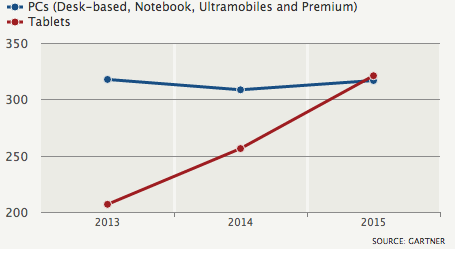
\includegraphics[width=0.50\textwidth]{tabletVsPC}
\label{fig:tabVsPC}
\caption{Worldwide Device Shipments (in millions) by Segment \cite{tabletOvertake}}
\end{figure}



\subsection{Android}\label{sec:Android}
The market share of the Android mobile operating system amongst mobile operating systems has been increasing steadily since 2012, going from 60\% in 2012 to 78\% in 2015 (see Fig \ref{fig:android}), which helped influence the decision to develop the application for Android so as to have the widest possible reach.

\begin{figure}[h]
\centering
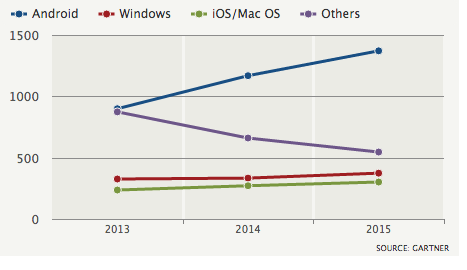
\includegraphics[width=0.50\textwidth]{android}\label{fig:android}\caption{Worldwide Device Shipments (in millions) by Operating System \cite{tabletOvertake}}
\end{figure}


 

\subsection{M-learning}


CodeTouch falls into the self-paced E-Learning market, which is a market currently experiencing constant growth and is expected to do so for the foreseeable future. Today it is worth £31.1 billion and is growing with a compound annual interest rate of 7.6\%.
Things get even more encouraging when examining the m-Education market, defined as any form of e-Learning delivered to a mobile device, which is currently worth £6.1 billion worldwide .The market has a projected compound annual interest rate of 20.65\% from 2013-2018 10, meaning in 2019 the sector is predicted to be worth £12.93 billion.


\section{}
why important? Writing code needs to catch up with the times, people are moving from desktops and laptos to tablets, big potential here especially with further development. 

Goals: provide basis of two products: firstly educational app. secondly, could be adapeted to work with real languages, could evolve into entire new way of programming

survey shows syntax mistakes are fustrating: put people off. People are very fickle with apps, (find percentage showing how many are used just once). less fustrating = more likely to keep playing : more livkely to catch coding fever etc

\section{Competitors}



\section{Target Audience}






This chapter should describe the project context, and motivate each of
the proposed aims and objectives.  Ideally, it is written at a fairly 
high-level, and easily understood by a reader who is technically 
competent but not an expert in the topic itself.

In short, the goal is to answer three questions for the reader.  First, 
what is the project topic, or problem being investigated?  Second, why 
is the topic important, or rather why should the reader care about it?  
For example, why there is a need for this project (e.g., lack of similar 
software or deficiency in existing software), who will benefit from the 
project and in what way (e.g., end-users, or software developers) what 
work does the project build on and why is the selected approach either
important and/or interesting (e.g., fills a gap in literature, applies
results from another field to a new problem).  Finally, what are the 
central challenges involved and why are they significant? 
 
The chapter should conclude with a concise bullet point list that 
summarises the aims and objectives.  For example:

\begin{quote}
\noindent

\subsection Motivation
This shift towards tablets from computers %\ref{shift}
, combined with the upturn of people interested in learning how to code%\ref{learnCode}, 
\begin{enumerate}
\item Help teachers to bridge the gap between visual code-block based coding and textual coding, a requirement of the new Key Stage 3 National Curriculum for Computing. 
\item Capitalise on coding's recent burst of popularity by designing an easy to use, intutive development environment for beginner programmers to learn the basics of programming.
\end{enumerate}
The high-level objective of this project is to create an coding application for Android devices, specifically tablets, where code is created via button presses. 

More specifically, the concrete aims are:

\begin{enumerate}
\item Help teachers to bridge the gap between visual code-block based coding and textual coding, a requirement of the new Key Stage 3 National Curriculum for Computing. 
\item Capitalise on coding's recent burst of popularity by designing an easy to use, intuitive development environment for beginner programmers to learn the basics of programming.
\item 

Design an interface for programming which allows text based code to be produced via button presses on a tablet rather than typing, capitalising on the social shift in popularity from Computers to tablets.  
\item Implement a framework for describing exponentiation algorithms
      and populate it with suitable examples from the literature on 
      an ARM7 platform.
\item Use the framework to perform a study of algorithm performance
      in terms of time and space, and show the proposed improvements
      are worthwhile.
\end{enumerate}
\end{quote}

% -----------------------------------------------------------------------------

\chapter{Technical Background}
\label{chap:technical}

\section{Supporting Technologies}
\subsection{Choice Between Developing A Native Application, Cross-Platform Application or Hybrid Application }
When deciding how to implement the application, there were three options to choose from:
\begin{enumerate}
\item \textbf{Native Application}
\begin{itemize}
A Native Application is written in a specific programming language for a specific hardware platform, for example Java for Android with Android, Objective C with iOS and C# for Windows Phone. Native apps are the best option in terms of performance as they can access the hardware of the device it is running on. Debugging is also easier, however the single platform nature of native applications make them more expensive to develop and maintain if cross platform coverage is desired, as companies need to do everything multiple times and potentially employ experts in multiple programming languages in order to maintain their app. 
\end{itemize}


\item \textbf{Cross-Platform Application}
\begin{itemize}
A Cross-Platform Application is an application written in a generic web language, most commonly HTML5, in order to be runnable on all mobile applications, which is an obvious advantage over developing nativley.  Other advantages include being able to update the application centrally, removing the need for the user to download updates.  However, having to accommodate for all different types of browser can cause maintenance problems, and the fact that Cross-Platform apps cannot be uploaded to the native Application stores (such as Apple's App Store and Google's Play Store) may put off potential users as the apps security cannot be verified. Furthermore, they do not perform as quickly as native apps and due to their cross-platform nature, have to look the same on all devices, which can make them look unnatural. 
\end{itemize}
\item \textbf {Hybrid Application}
\begin{itemize}
A Hybrid Application aims to  combine the advantages of native and web app development. They are developed in generic web languages but are wrapped in native code. This means they can be cross platform but still take advantage of the devices in-built features. However, they still retain the disadvantages of cross-platform apps in that they do not perform as well and can look unnatural.
\end{itemize}
\end{enumerate}

For CodeTouch, the performance of the application is very critical to the applications core function; when a user is creating code, it should feel instant and natural. Seeing as it was difficult to predict if there would be any performance issues before development on the application started, the decision was made to go native in order to minimise the risk of poor performance affecting the application's use-ability. Once this decision was made, the decision to go for Android was made based on reasons articulated earlier in this document (see \ref{sec:Android});









Talk about history of language engineering, of real time error checking


Talk in depth how code block programming works

Talk in depth how code academy works

Talk in depth how CodeTouch meets in the middel

Talk about touch develop: sort of bridges gap but not quite, doesn't have flow of writing code like CodeTouch

talk about pencil code

Output is real code, looks like java but could be tweaked to be anything, or indeed to actually create valid java.

\noindent
This chapter is intended to describe the technical basis on which execution
of the project depends.  The goal is to provide a detailed explanation of
the specific problem at hand, and existing work that is relevant (e.g., an
existing algorithm that you use, alternative solutions proposed, supporting
technologies).  

Per the same advice in the handbook, note there is a subtly difference from
this and a full-blown literature review (or survey).  The latter might try
to capture and organise (e.g., categorise somehow) {\em all} related work,
potentially offering meta-analysis, whereas here the goal is simple to
ensure the dissertation is self-contained.  Put another way, after reading 
this chapter a non-expert reader should have obtained enough background to 
understand what {\em you} have done, and then accurately assess your work.
You might view an additional goal as giving the reader confidence that you 
are able to absorb, understand and clearly communicate highly technical 
material.

% -----------------------------------------------------------------------------

\chapter{Project Execution}
\label{chap:execution}

{\bf A topic-specific chapter, of roughly $20$ pages} 
\vspace{1cm} 

\noindent
This chapter is intended to describe what you did: the goal is to explain
the main activity or activities, of any type, which constituted your work 
during the project.  The content is highly topic-specific, but for many 
projects it will make sense to split the chapter into two sections: one 
will discuss the design of something (e.g., some hardware or software, or 
an algorithm, or experiment), including any rationale or decisions made, 
and the other will discuss how this design was realised via some form of 
implementation.  

This is, of course, far from ideal for {\em many} project topics.  Some
situations which clearly require a different approach include:

\begin{itemize}
\item In a project where asymptotic analysis of some algorithm is the goal,
      there is no real ``design and implementation'' in a traditional sense
      even though the activity of analysis is clearly within the remit of
      this chapter.
\item In a project where analysis of some results is as major, or a more
      major goal than the implementation that produced them, it might be
      sensible to merge this chapter with the next one: the main activity 
      is such that discussion of the results cannot be viewed separately.
\end{itemize}

\noindent
Note that it is common to include evidence of ``best practice'' project 
management (e.g., use of version control, choice of programming language 
and so on).  Rather than simply a rote list, make sure any such content 
is useful and/or informative in some way: for example, if there was a 
decision to be made then explain the trade-offs and implications 
involved.

\section{Example Section}

This is an example section; 
the following content is auto-generated dummy text.
\lipsum

\subsection{Example Sub-section}

\begin{figure}[t]
\centering
foo
\caption{This is an example figure.}
\label{fig}
\end{figure}

\begin{table}[t]
\centering
\begin{tabular}{|cc|c|}
\hline
foo      & bar      & baz      \\
\hline
$0     $ & $0     $ & $0     $ \\
$1     $ & $1     $ & $1     $ \\
$\vdots$ & $\vdots$ & $\vdots$ \\
$9     $ & $9     $ & $9     $ \\
\hline
\end{tabular}
\caption{This is an example table.}
\label{tab}
\end{table}

\begin{algorithm}[t]
\For{$i=0$ {\bf upto} $n$}{
  $t_i \leftarrow 0$\;
}
\caption{This is an example algorithm.}
\label{alg}
\end{algorithm}

\begin{lstlisting}[float={t},caption={This is an example listing.},label={lst},language=C]
for( i = 0; i < n; i++ ) {
  t[ i ] = 0;
}
\end{lstlisting}

This is an example sub-section;
the following content is auto-generated dummy text.
Notice the examples in Figure~\ref{fig}, Table~\ref{tab}, Algorithm~\ref{alg}
and Listing~\ref{lst}.
\lipsum

\subsubsection{Example Sub-sub-section}

This is an example sub-sub-section;
the following content is auto-generated dummy text.
\lipsum

\paragraph{Example paragraph.}

This is an example paragraph; note the trailing full-stop in the title,
which is intended to ensure it does not run into the text.

% -----------------------------------------------------------------------------

\chapter{Critical Evaluation}
\label{chap:evaluation}

{\bf A topic-specific chapter, of roughly $10$ pages} 
\vspace{1cm} 

\noindent
This chapter is intended to evaluate what you did.  The content is highly 
topic-specific, but for many projects will have flavours of the following:

TALK ABOUT how i could have used reverse shunting algorithm for brackets expression, explain it in depth

IDEA colaberative programming for classroom, so every pupil could have tablet with code, teacher chooses person to do next line

\begin{enumerate}
\item functional  testing, including analysis and explanation of failure 
      cases,
\item behavioural testing, often including analysis of any results that 
      draw some form of conclusion wrt. the aims and objectives,
      and
\item evaluation of options and decisions within the project, and/or a
      comparison with alternatives.
\end{enumerate



\noindent
This chapter often acts to differentiate project quality: even if the work
completed is of a high technical quality, critical yet objective evaluation 
and comparison of the outcomes is crucial.  In essence, the reader wants to
learn something, so the worst examples amount to simple statements of fact 
(e.g., ``graph X shows the result is Y''); the best examples are analytical 
and exploratory (e.g., ``graph X shows the result is Y, which means Z; this 
contradicts , which may be because I use a different assumption'').  As 
such, both positive {\em and} negative outcomes are valid {\em if} presented 
in a suitable manner.

% -----------------------------------------------------------------------------

\chapter{Conclusion}
\label{chap:conclusion}

{\bf A compulsory chapter, of roughly $2$ pages} 
\vspace{1cm} 

\noindent
The concluding chapter of a dissertation is often underutilised because it 
is too often left too close to the deadline: it is important to allocation
enough attention.  Ideally, the chapter will consist of three parts:

\begin{enumerate}
\item (Re)summarise the main contributions and achievements, in essence
      summing up the content.
\item Clearly state the current project status (e.g., ``X is working, Y 
      is not'') and evaluate what has been achieved with respect to the 
      initial aims and objectives (e.g., ``I completed aim X outlined 
      previously, the evidence for this is within Chapter Y'').  There 
      is no problem including aims which were not completed, but it is 
      important to evaluate and/or justify why this is the case.
\item Outline any open problems or future plans.  Rather than treat this
      only as an exercise in what you {\em could} have done given more 
      time, try to focus on any unexplored options or interesting outcomes
      (e.g., ``my experiment for X gave counter-intuitive results, this 
      could be because Y and would form an interesting area for further 
      study'' or ``users found feature Z of my software difficult to use,
      which is obvious in hindsight but not during at design stage; to 
      resolve this, I could clearly apply the technique of Smith [7]'').
\end{enumerate}

% =============================================================================

% Finally, after the main matter, the back matter is specified.  This is
% typically populated with just the bibliography.  LaTeX deals with these
% in one of two ways, namely
%
% - inline, which roughly means the author specifies entries using the 
%   \bibitem macro and typesets them manually, or
% - using BiBTeX, which means entries are contained in a separate file
%   (which is essentially a databased) then inported; this is the 
%   approach used below, with the databased being dissertation.bib.
%
% Either way, the each entry has a key (or identifier) which can be used
% in the main matter to cite it, e.g., \cite{X}, \cite[Chapter 2}{Y}.

\backmatter

\bibliography{dissertation}


% -----------------------------------------------------------------------------

% The dissertation concludes with a set of (optional) appendicies; these are 
% the same as chapters in a sense, but once signaled as being appendicies via
% the associated macro, LaTeX manages them appropriatly.

\appendix

\chapter{An Example Appendix}
\label{appx:example}



Content which is not central to, but may enhance the dissertation can
be included in one or more appendices; examples include, but are not 
limited to

\begin{itemize}
\item lengthy mathematical proofs, numerical or graphical results
      which are summarised in the main body,
\item sample or example calculations, 
      and
\item results of user studies or questionnaires.
\end{itemize}


\noindent
Note that in line with most research conferences, the marking panel 
is not obliged to read such appendices.

% =============================================================================
\subsection{Survey Results}
\label{ssec:survey}
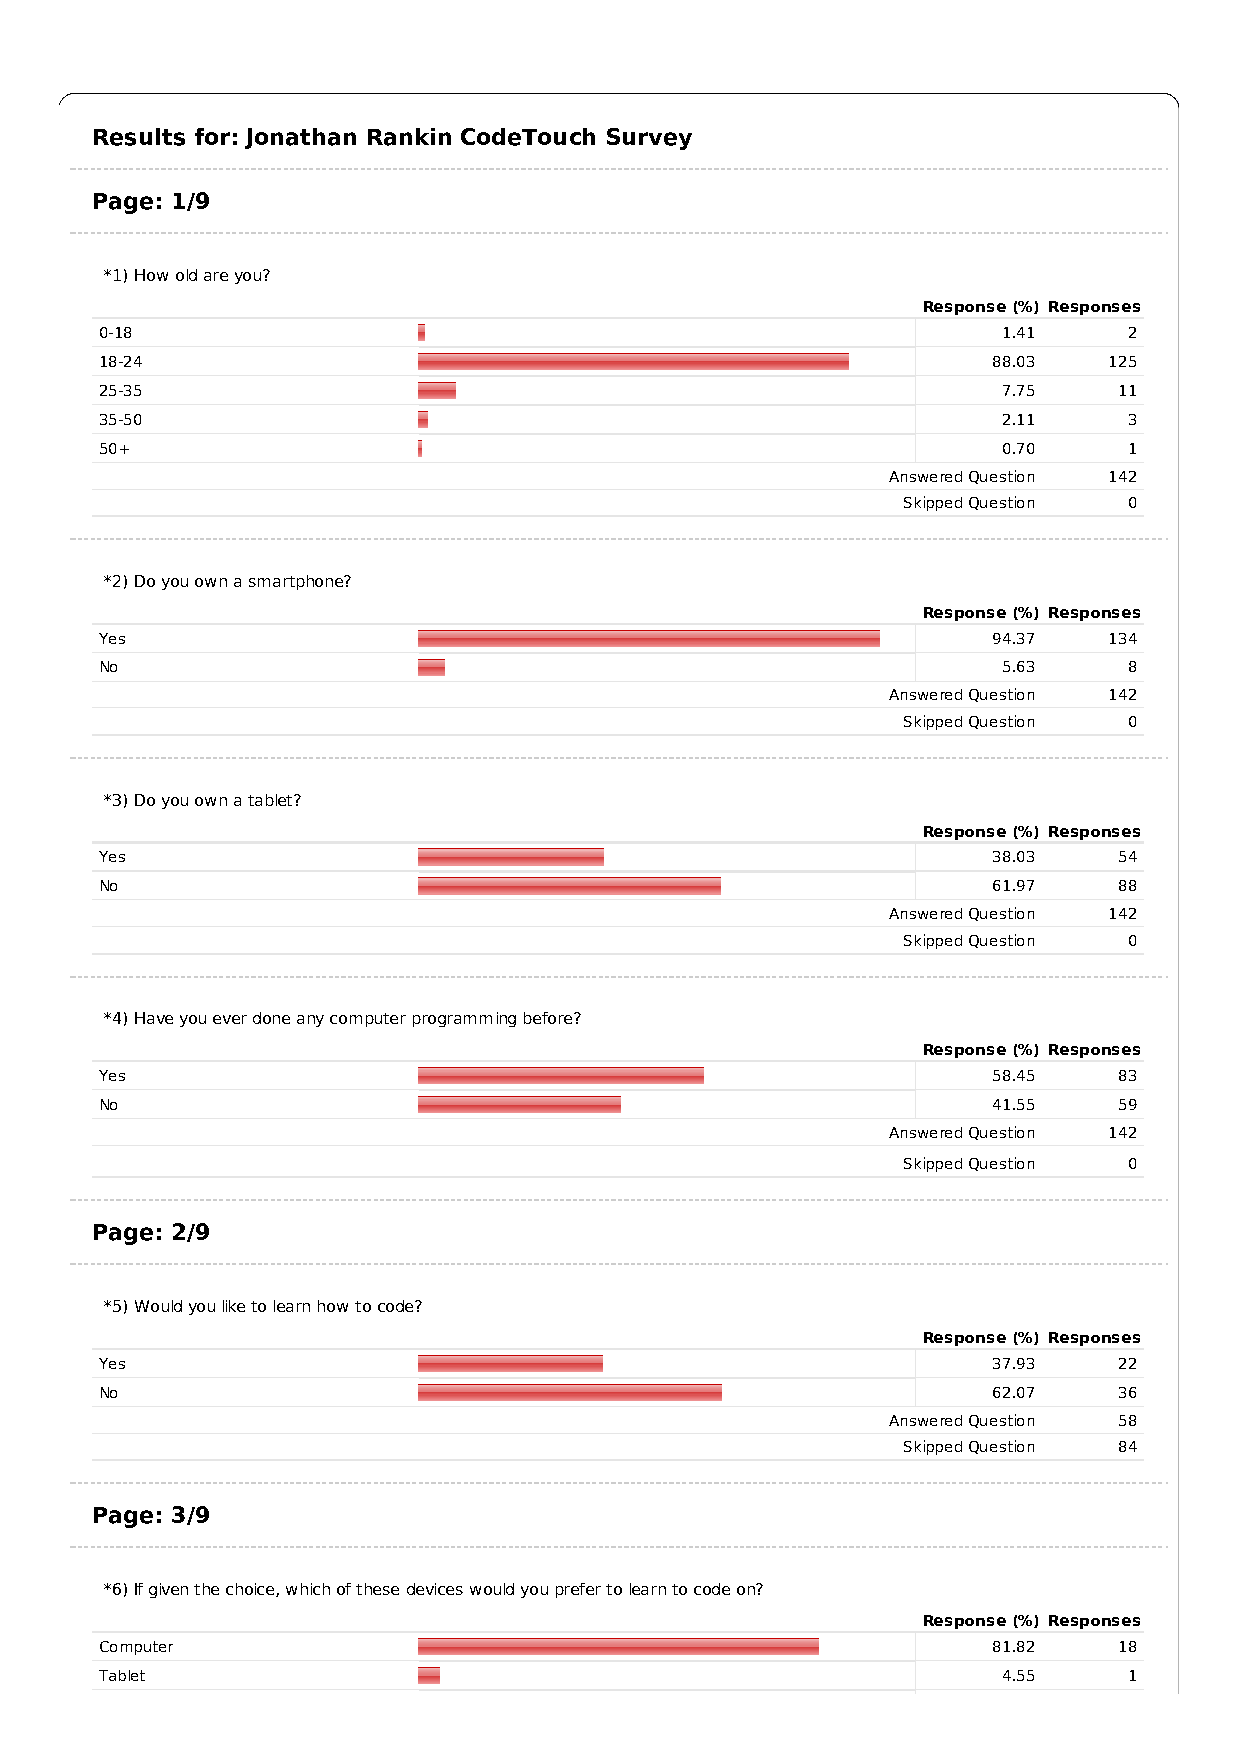
\includepdf[pages={1-6}]{survey.pdf}

\end{document}
